% CSD311 Artificial Intelligence -- group project report.
% Compile with pdflatex + bibtex (e.g. upload the report/ folder to Overleaf):
%   pdflatex main && bibtex main && pdflatex main && pdflatex main
\documentclass[11pt,a4paper]{article}

\usepackage[T1]{fontenc}
\usepackage[utf8]{inputenc}
\usepackage{lmodern}
\usepackage[margin=2.5cm]{geometry}
\usepackage{amsmath,amssymb}
\usepackage{graphicx}
\usepackage{booktabs}
\usepackage{tabularx}
\usepackage{multirow}
\usepackage{array}
\usepackage{caption}
\usepackage{placeins}
\usepackage{enumitem}
\usepackage{xcolor}
\usepackage{tikz}
\usetikzlibrary{arrows.meta,positioning,calc}
\usepackage[hidelinks]{hyperref}

% Let a text page hold more floats, so tables stay close to their text.
\renewcommand{\topfraction}{0.85}
\renewcommand{\bottomfraction}{0.6}
\renewcommand{\textfraction}{0.1}
\renewcommand{\floatpagefraction}{0.75}
\setcounter{totalnumber}{4}

\captionsetup{font=small,labelfont=bf}
\setlist{itemsep=2pt,topsep=4pt}
\graphicspath{{figures/}}

\newcommand{\bd}[2]{$#1{\times}#2$}            % board size, e.g. \bd{3}{3}
\newcommand{\outside}{\textsuperscript{$\dagger$}} % technique from outside the course
\newcommand{\code}[1]{\texttt{#1}}

\begin{document}

% ---------------------------------------------------------------- title page
\begin{titlepage}
\fontfamily{ptm}\selectfont % Times, as in the group's report template
\centering
\vspace*{0.4cm}
{\Large\bfseries Shiv Nadar University\par}
\vspace{0.25cm}
{\large Computer Science Department\par}
\vspace{1.5cm}
{\large\bfseries Artificial Intelligence (CSD311)\par}
\vspace{0.2cm}
{\large Final Group Project Report\par}
\vspace{1.5cm}
\rule{\linewidth}{1.2pt}\par
\vspace{1.3cm}
{\fontsize{26}{32}\selectfont\bfseries Dots and Boxes\par}
\vspace{1.3cm}
\rule{\linewidth}{1.2pt}\par
\vspace{1.5cm}
{\large\itshape Submitted by\par}
\vspace{0.3cm}
{\large\renewcommand{\arraystretch}{1.3}%
\begin{tabularx}{0.72\linewidth}{>{\centering\arraybackslash}X>{\centering\arraybackslash}X}
\toprule[1.2pt]
\textbf{Group Member} & \textbf{Roll Number} \\
\midrule[0.4pt]
Daksh Jain & 2410110113 \\
Tilika Chopra & 2410110361 \\
Arnav Jyoti & 2410110071 \\
Abhyuday Aulakh & 2410110016 \\
Dev Khemani & 2410110119 \\
Medhavee Binnani & 2410110198 \\
Disha Singh & 2410110128 \\
Vaidehi Saxena & 2410110366 \\
\end{tabularx}\par}
\vspace{1.5cm}
{\large\itshape Submitted to\par}
\vspace{0.25cm}
{\large\bfseries Snehasis Mukherjee\par}
\vspace{1.2cm}
{\large Submission date: 16 November 2026\par}
\end{titlepage}

% ---------------------------------------------------------------- abstract
\begin{abstract}
\noindent
We build seven independent players for the game of Dots and Boxes, one per family of
techniques from the CSD311 course, on a shared game engine, feature extractor and
tournament harness: Random and Greedy baselines, an exact solver (negamax with
memoisation, symmetry reduction and alpha-beta pruning), a heuristic search player
(iterative-deepening alpha-beta with a transposition table, move ordering and
quiescence), a rule-based player written in Prolog (with an equivalent Python version),
Monte Carlo players (flat Monte
Carlo and UCT), search players whose evaluation weights are tuned by four metaheuristics
(genetic algorithm, hill climbing, simulated annealing and tabu search), and supervised
learners (kNN, perceptron, sigmoid unit, multilayer perceptron, SVM, naive Bayes and a
decision tree). Every search method handles the extra-turn rule, which breaks the
usual alternation of turns. Six seeded experiments compare them. The exact solver
shows that the first player loses \bd{3}{3} by three boxes under perfect play, and
alpha-beta with symmetry cuts the nodes needed to solve \bd{2}{3} by $8.8\times$. In a
3{,}300-game round robin on \bd{3}{3}, untuned heuristic search is strongest (win rate
0.76), search with a learned evaluation is second (0.72), and the tuned players follow
(0.64--0.68). Tuning beats the hand-set weights at the depth it was run at, but the gain
does not survive deeper search, and on larger boards we trace a collapse of the tuned
players to raw-count features whose scale grows with the board. A $64{\times}64$ MLP
picks an optimal move in 97.2\% of \bd{2}{3} test positions; flat Monte Carlo beats UCT
at every budget, which we attribute to rollouts that never double-deal.

\medskip\noindent\textbf{Keywords:} Dots and Boxes, adversarial search, alpha-beta pruning,
Monte Carlo tree search, knowledge-based agents, metaheuristic optimisation, supervised
learning.
\end{abstract}

% ---------------------------------------------------------------- introduction
\section{Introduction}

Dots and Boxes is a two-player game played on a grid of $(m+1)\times(n+1)$ dots, that is,
$m\times n$ boxes. Players take turns drawing one undrawn line between two adjacent dots.
Drawing the fourth side of a box claims it, and a player who claims at least one box
must move again. The game ends when every line is drawn, and the player with more boxes
wins. The game is simple to state, yet expert play rests on deep combinatorial theory:
long chains of boxes, the long chain rule and the sacrifice known as double-dealing
\cite{berlekamp2000dots,berlekamp2003winning}.

The game is a good testbed for AI techniques for three reasons. First, the
\emph{extra-turn rule} means turns do not strictly alternate, so standard minimax,
alpha-beta and Monte Carlo tree search must be adapted rather than copied. Second, small
boards can be solved exactly, which gives a ground truth against which every other
player can be scored. Third, the strategic structure (chains and loops) can be written
as explicit rules, learned from data, or discovered by search, so the same game supports
deductive, inductive and search-based players.

This project builds one player per technique family taught in CSD311 \cite{csd311notes},
plus standard techniques from outside the course, marked with \outside\ and cited.
All players share one engine, one feature vector and one tournament harness, so they can
be compared head-to-head under identical conditions. The contributions are:
\begin{itemize}
\item seven solvers (Section~\ref{sec:method}) with a common value convention for the
  extra-turn rule;
\item six seeded experiments (Section~\ref{sec:results}): overall strength, search
  efficiency, an optimiser comparison under an equal evaluation budget, learned
  evaluators, deductive against inductive play, and Monte Carlo scaling;
\item two findings about tuned evaluation functions: weights tuned at a fixed shallow
  depth do not carry over to deeper search, and weights on raw counts break down as the
  board grows; we explain the mechanism behind both.
\end{itemize}

% ---------------------------------------------------------------- literature survey
\section{Literature Survey}

\paragraph{Combinatorial theory of Dots and Boxes.}
Berlekamp, Conway and Guy analysed Dots and Boxes as a combinatorial game in
\emph{Winning Ways} \cite{berlekamp2003winning}, and Berlekamp's book
\cite{berlekamp2000dots} develops the practical strategy: once no safe move is left,
players must open chains and loops; the player in \emph{control} takes all but two boxes
of each long chain (four of each loop) and declines the rest with a
\emph{double-dealing} move, forcing the opponent to open the next component. The
\emph{long chain rule} predicts who gets control: the first player wants the number of
dots plus long chains to be even. Our rule-based player and our parity feature encode
this theory.

\paragraph{Solving games.}
Allis \cite{allis1994searching} surveys how games are solved by search, with
transposition tables and symmetry as the main tools. Barker and Korf
\cite{barker2012solving} solved the \bd{4}{5} Dots and Boxes board by alpha-beta search
with a transposition table and symmetry reduction, among other enhancements. Our exact
solver applies the same ideas at a smaller scale and confirms the value of \bd{3}{3}.

\paragraph{Adversarial search.}
Minimax with alpha-beta pruning \cite{knuth1975alphabeta,russell2020aima} is the
standard method for two-player games. Iterative deepening \cite{korf1985iddfs} turns
depth-limited search into an anytime algorithm, and transposition tables with the
previous iteration's best move searched first come from early chess programs
\cite{slate1977chess}. Quiescence search extends the search along forcing lines (here,
captures) to avoid the horizon effect \cite{russell2020aima}. We adapt all of these to
the extra-turn rule.

\paragraph{Monte Carlo methods.}
Flat Monte Carlo evaluates each move by random playouts \cite{brugmann1993montecarlo}.
Monte Carlo tree search \cite{coulom2006efficient} grows a tree selectively, and UCT
\cite{kocsis2006bandit} selects children with an upper confidence bound; Browne et al.\
\cite{browne2012survey} survey the family. For Dots and Boxes specifically, Zhuang et
al.\ \cite{zhuang2015dotsboxes} improved MCTS with a novel board representation and
neural networks, which motivates our analysis of why plain UCT struggles on this game.

\paragraph{Tuning and learning evaluation functions.}
Samuel's checkers program \cite{samuel1959checkers} already tuned a weighted evaluation
function automatically. Metaheuristics offer general tools for such tuning: genetic
algorithms \cite{holland1975adaptation} with real-coded BLX crossover
\cite{eshelman1993blx}, simulated annealing \cite{kirkpatrick1983annealing} with the
Metropolis acceptance rule \cite{metropolis1953equation}, tabu search \cite{glover1989tabu}
and hill climbing \cite{russell2020aima}. Learning an evaluation from data goes back to
TD-Gammon \cite{tesauro1995tdgammon} and, combined with search, to AlphaGo
\cite{silver2016alphago}. Our supervised learners use the classical models of the
course: the perceptron \cite{rosenblatt1958perceptron}, multilayer networks trained by
backpropagation \cite{rumelhart1986backprop}, nearest neighbours \cite{cover1967nearest},
support vector machines \cite{cortes1995svm} and decision trees \cite{quinlan1986id3},
and we examine the bias--variance trade-off \cite{geman1992biasvariance}.

% ---------------------------------------------------------------- method
\section{Method}
\label{sec:method}

Techniques from outside the course syllabus are marked \outside; the rest follow the
CSD311 lecture notes \cite{csd311notes}.

\subsection{Problem formulation}

The task is to choose, in any legal position of an $m\times n$ game, the edge that
maximises the mover's final box margin against an adversary. In the terms of
\cite{russell2020aima}, the environment is fully observable, deterministic, sequential,
static, discrete and two-agent competitive, and the game is an adversarial search problem:
\begin{itemize}
\item \textbf{State:} the set of drawn edges, the two scores and the player to move. On
  \bd{2}{2}, \bd{2}{3} and \bd{3}{3} there are $2^{12}=4{,}096$, $2^{17}=131{,}072$ and
  $2^{24}\approx 16.8$ million edge configurations.
\item \textbf{Initial state:} no edge drawn, scores $(0,0)$, player 0 to move.
\item \textbf{Actions:} any undrawn edge, so the branching factor equals the number of
  undrawn edges and falls by one with every move.
\item \textbf{Transition model:} drawing an edge completes $k\in\{0,1,2\}$ boxes; if $k>0$
  the mover scores $k$ and moves again, otherwise the turn passes.
\item \textbf{Terminal test and utility:} the game ends when every edge is drawn; the
  utility is the box difference, so the game is zero-sum.
\end{itemize}

\subsection{System architecture}

The system has three layers (Figure~\ref{fig:arch}). The foundation is the game engine
(board tables, rules, symmetry and chain analysis) and the shared feature extractor. The
middle layer holds the seven solvers, each a subclass of one abstract \code{Player} class
whose \code{choose\_move(state, time\_limit)} returns a legal edge. The top layer creates
players by name and lets them play: the tournament harness, the experiment scripts, an
interactive application and the test suite. Code is shared so that comparisons are fair:
Greedy's move function is the Monte Carlo rollout policy; its capture routine is also the
quiescence step of the search player and the sacrifice estimate of the rule player; the
chain analysis serves both the features and the rules; and the search player accepts
either a weight vector or any evaluation function, which is how the tuned (solver 6) and
learned (solver 7) variants reuse solver 3 without copying it.

\begin{figure}[htbp]
\centering
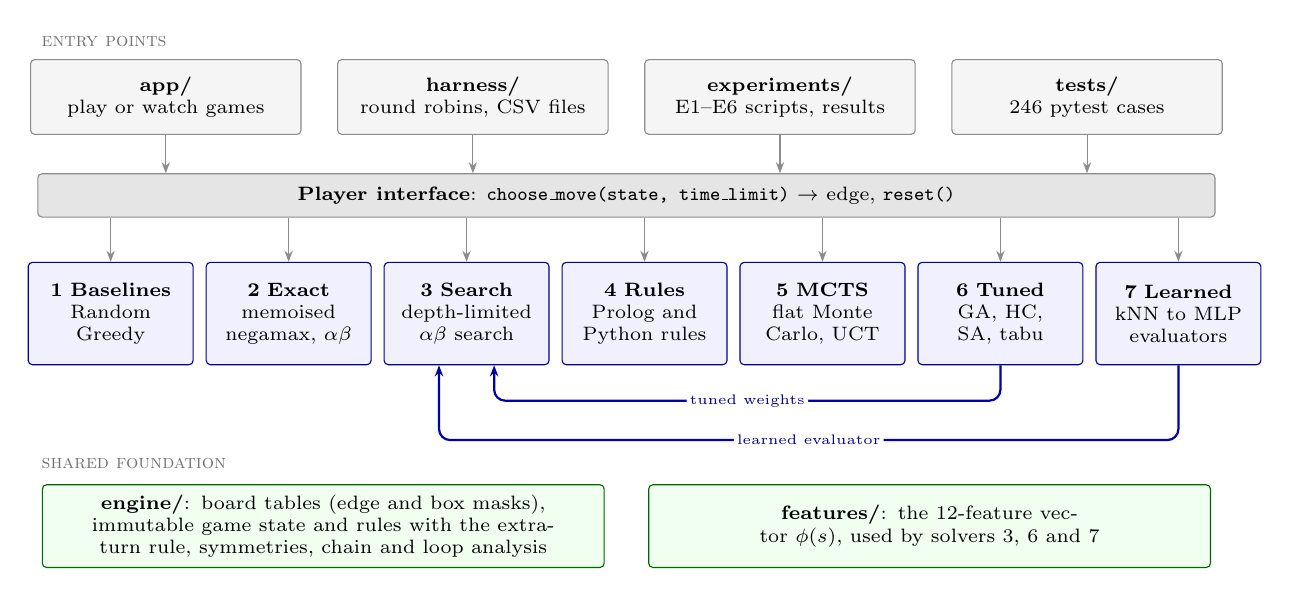
\begin{tikzpicture}[
  font=\scriptsize, >={Stealth[length=4pt]},
  every node/.style={align=center},
  layer/.style={font=\scriptsize\scshape, text=black!55, anchor=west},
  entry/.style={draw=black!45, fill=black!4, rounded corners=1.5pt, minimum height=0.95cm, text width=3.2cm},
  solver/.style={draw=blue!55!black, fill=blue!6, rounded corners=1.5pt, minimum height=1.3cm, text width=1.86cm},
  found/.style={draw=green!40!black, fill=green!6, rounded corners=1.5pt, minimum height=1.05cm, text width=6.9cm},
  reuse/.style={->, draw=blue!65!black, thick, rounded corners=4pt},
  lab/.style={font=\tiny, text=blue!55!black, fill=white, inner sep=1.2pt}]
% entry points
\node[layer] at (-0.15, 4.3) {entry points};
\node[entry] (app) at (1.55, 3.6) {\textbf{app/}\\ play or watch games};
\node[entry] (har) at (5.45, 3.6) {\textbf{harness/}\\ round robins, CSV files};
\node[entry] (exp) at (9.35, 3.6) {\textbf{experiments/}\\ E1--E6 scripts, results};
\node[entry] (tst) at (13.25, 3.6) {\textbf{tests/}\\ 246 pytest cases};
% player interface
\node[draw=black!45, fill=black!10, rounded corners=1.5pt, minimum width=14.95cm, minimum height=0.55cm]
  (api) at (7.4, 2.35) {\textbf{Player interface}: \code{choose\_move(state, time\_limit)} $\rightarrow$ edge, \code{reset()}};
% solvers
\node[solver] (s1) at (0.85, 0.85) {\textbf{1 Baselines}\\ Random\\ Greedy};
\node[solver] (s2) at (3.11, 0.85) {\textbf{2 Exact}\\ memoised\\ negamax, $\alpha\beta$};
\node[solver] (s3) at (5.37, 0.85) {\textbf{3 Search}\\ depth-limited\\ $\alpha\beta$ search};
\node[solver] (s4) at (7.63, 0.85) {\textbf{4 Rules}\\ Prolog and\\ Python rules};
\node[solver] (s5) at (9.89, 0.85) {\textbf{5 MCTS}\\ flat Monte\\ Carlo, UCT};
\node[solver] (s6) at (12.15, 0.85) {\textbf{6 Tuned}\\ GA, HC,\\ SA, tabu};
\node[solver] (s7) at (14.41, 0.85) {\textbf{7 Learned}\\ kNN to MLP\\ evaluators};
\foreach \x in {app,har,exp,tst} { \draw[->, black!45] (\x.south) -- (\x.south |- api.north); }
\foreach \i in {1,...,7} { \draw[->, black!45] (api.south -| s\i) -- (s\i.north); }
% reuse into solver 3: nested levels, so the two paths never cross
\draw[reuse] (s6.south) -- ++(0,-0.45) -| node[lab, pos=0.25] {tuned weights} ($(s3.south)+(0.35,0)$);
\draw[reuse] (s7.south) -- ++(0,-0.95) -| node[lab, pos=0.25] {learned evaluator} ($(s3.south)+(-0.35,0)$);
% foundation
\node[layer] at (-0.15, -1.05) {shared foundation};
\node[found] (eng) at (3.55, -1.85) {\textbf{engine/}: board tables (edge and box masks), immutable game
  state and rules with the extra-turn rule, symmetries, chain and loop analysis};
\node[found] (fea) at (11.25, -1.85) {\textbf{features/}: the 12-feature vector $\phi(s)$, used by
  solvers 3, 6 and 7};
\end{tikzpicture}
\caption{System architecture. Every solver implements one \code{Player} interface on top of the
engine. Blue arrows show solvers 6 and 7 reusing solver 3; in addition, solver 1's Greedy policy is
solver 5's rollout policy, and solvers 2 and 5 label the training data of solver 7.}
\label{fig:arch}
\end{figure}

The project is about 6{,}000 lines of Python, 260 lines of Prolog and 2{,}300 lines of
tests. A position's drawn edges are one Python integer, and the engine
precomputes a mask of the four edges of each box, so counting a box's drawn sides is one
population count and a move is one bitwise OR. States are immutable, which makes them
safe to share between the search, the application's user-interface thread and the tests.
Every stochastic component takes an explicit seed, and the test suite checks the exact
solver against an unmemoised brute force and an independent retrograde table, the chain
analysis and each rule on hand-drawn positions, the search against plain negamax, and
time-limit compliance.

\subsection{Game representation and value convention}

A board of $m\times n$ boxes has $H=(m+1)n$ horizontal and $V=m(n+1)$ vertical edges,
$E=H+V$ in total (24 on \bd{3}{3}, 40 on \bd{4}{4}). A position is an $E$-bit integer
with bit $i$ set when edge $i$ is drawn, together with the scores and the player to move;
lookup tables give the four edges of each box and the one or two boxes of each edge. All
hot loops (search, rollouts) work on the raw bitmask.

All values are from the point of view of the \emph{player to move} and count the net
boxes still to be gained, excluding boxes already scored. For a move $a$ that completes
$k$ boxes and leads to $s'$,
\begin{equation}
  \mathrm{value}(s,a) =
  \begin{cases}
    k + V(s') & \text{if } k>0 \text{ (same player again)},\\
    -V(s')    & \text{if } k=0 \text{ (turn passes)},
  \end{cases}
  \qquad V(\text{terminal}) = 0 .
  \label{eq:value}
\end{equation}
Alpha-beta windows follow the same rule: after a capture the child is searched with the
window $(\alpha-k,\beta-k)$ without negation; otherwise with $(-\beta,-\alpha)$, negated.
This one convention is shared by the exact solver, heuristic search, the Monte Carlo
rewards and the learned evaluators.

\subsection{Shared features}

The heuristic, tuned and learned players use one 12-dimensional feature vector
$\phi(s)$: the numbers of boxes with 0, 1, 2 and 3 sides drawn; the number of safe moves
(moves that give no box its third side); the number of long chains ($\geq 3$ boxes) and
the boxes in them; the number of short chains; the number of loops and the boxes in
them; a long-chain parity indicator ($+1$ if dots plus long chains has the parity the
player to move wants \cite{berlekamp2000dots}, $-1$ otherwise); and the fraction of edges
drawn. Chains and loops come from a shared chain analysis: a chain is a maximal sequence
of 2-sided boxes connected through undrawn edges, and a loop is a chain that closes on
itself.

\subsection{Solver 1: Random and Greedy baselines}

Random plays a uniformly random legal move. Greedy is a best-first policy: it captures
whenever it can (a double capture first), otherwise plays a random safe move, and when
none is left it plays the sacrifice after which the opponent's capture run is shortest.
Greedy never double-deals, which is exactly what chain strategy exploits. It is also the
rollout policy of the Monte Carlo players and the reference opponent in most experiments.

\subsection{Solver 2: Exact solver}

The exact solver computes $V$ of Eq.~\eqref{eq:value} by depth-first negamax. Because $V$
depends only on the edges, results are memoised in a transposition table (node marking).
Two optional speed-ups are compared in E2: \emph{symmetry reduction}\outside, keying the
table on the smallest image of the position under the 8 symmetries of a square board (4
of a rectangle), and \emph{alpha-beta pruning}\outside\ \cite{knuth1975alphabeta} with
table entries flagged as exact, lower or upper bounds. The solver plays perfectly on
small boards, labels datasets for solver 7 and scores the other players' moves.
Memoisation bounds the work by the number of distinct positions: each of the $2^E$ edge
masks is expanded once, so the solver needs $O(E\cdot 2^E)$ time and $O(2^E)$ memory,
against about $E!$ move sequences without it.

\subsection{Solver 3: Heuristic search}

Solver 3 is depth-limited negamax with alpha-beta pruning\outside\ under the extra-turn
windows, run by iterative deepening \cite{korf1985iddfs}. At the depth cutoff it scores
a position with $h(s)=w\cdot\phi(s)$, where the hand-set weights put $1$ on capturable
boxes and $1.5$ on the parity indicator and $0$ elsewhere. Three enhancements are tested
in E2: a transposition table\outside\ with bound flags, move ordering\outside\ (double
captures, captures, safe moves, then sacrifices, with the table's or previous
iteration's best move first) and quiescence\outside, which plays out all pending captures
before evaluating. Iterative deepening stops when the next iteration, predicted as the
last one's time multiplied by its effective branching factor $b^*$, would overrun the
time limit. $b^*$ solves $N=b^*+b^{*2}+\dots+b^{*d}$ for $N$ nodes at depth $d$
\cite{csd311notes}. With perfect move ordering, alpha-beta examines about $b^{d/2}$ nodes
instead of $b^d$ \cite{knuth1975alphabeta}; $b^*$ measures how close the implementation
comes to that.

\subsection{Solver 4: Rule-based player}

Solver 4 is the deductive player. Board facts (edges, box sides, dots, drawn edges, the
player to move) are asserted into SWI-Prolog \cite{wielemaker2012swipl,clocksin2003prolog},
chains are found by a recursive relation over linked 2-sided boxes, and a cut commits to
the first rule that applies:
\begin{enumerate}
\item \emph{Endgame double-deal}\outside: when the opponent has opened a long chain or
  loop and other long components remain, take all but two boxes (four for a loop) and
  decline the rest, unless the sacrifice exceeds the estimated value of keeping control;
\item \emph{capture} any other capturable box;
\item \emph{parity-steering safe move}\outside: a safe move after which the long chain
  rule favours this player;
\item any \emph{safe move};
\item \emph{minimum sacrifice}: open the component that gives away fewest boxes, opening
  a 2-chain by its middle edge (a hard-hearted handout\outside) so the opponent cannot
  double-deal.
\end{enumerate}
A pure-Python backend implements the same rules move for move; a test checks that both
backends agree, and the experiments use the Python backend for speed.

\subsection{Solver 5: Monte Carlo players}

\emph{Flat Monte Carlo} spreads rollouts evenly over the legal moves and plays the move
with the best mean reward. \emph{UCT}\outside\ \cite{kocsis2006bandit} grows a tree. Each
iteration descends from the root by choosing the child $j$ that maximises
\begin{equation}
  \mathrm{UCT}_j = \frac{W_j}{n_j} + c\sqrt{\frac{\ln N}{n_j}},
  \label{eq:uct}
\end{equation}
where $W_j$ and $n_j$ are the child's total reward and visits and $N$ its parent's visits,
then expands one untried move, plays a rollout to the end of the game and backs the result
up the path. One iteration costs $O(E^2)$ time, since a rollout makes up to $E$ Greedy
moves that each scan the edges. Rollouts follow Greedy with
probability $1-\varepsilon$ and a random move otherwise ($\varepsilon=0.1$). The reward is
the normalised margin $(\mathit{net}+B)/2B$ over the $B$ boxes, measured from the root
onward. Because of the extra-turn rule, every node stores its reward from the view of
the player who made the move into it (the parent's player to move), never by assuming
alternation. The tree is reused between moves only along non-capturing moves, since
rewards are measured from the root. Defaults ($c=0.5$, margin reward) were chosen by
tuning on \bd{2}{2} and \bd{3}{3}; the margin reward beat a win/loss reward because the
latter cannot tell a 2-box loss from a 4-box loss.

\subsection{Solver 6: Metaheuristic-tuned evaluation}

Solver 6 tunes the 12 weights $w\in[-5,5]^{12}$ of solver 3. The fitness of $w$ is
measured by 40 games at search depth 2, half against Greedy and half against untuned
depth-2 search, with the first player alternating and the same seeds for every $w$
(common random numbers):
\begin{equation}
  f(w) = \overline{\text{win}} + 0.01\,\overline{\text{margin}}/\text{boxes},
\end{equation}
with a draw counting $0.5$. Identical weight vectors are cached. Every optimiser gets the
same budget of 600 fitness evaluations (cache hits included), as the course warns against
comparing by generations:
\begin{itemize}
\item \textbf{Genetic algorithm} \cite{holland1975adaptation}: population 20 seeded with
  the hand-set weights, tournament selection ($q=3$), BLX-0.5 crossover
  \cite{eshelman1993blx} at rate 0.9, Gaussian mutation ($\sigma=0.3$, rate $1/12$ per
  gene), elitism of 2.
\item \textbf{Hill climbing}: stochastic; perturbs one random weight by
  $\mathcal{N}(0,0.5^2)$ and accepts only improvements, restarting from a random point
  once 30 perturbations have failed since the last restart.
\item \textbf{Simulated annealing} \cite{kirkpatrick1983annealing}: the same moves,
  accepting a worse move with probability $e^{\Delta/T}$ \cite{metropolis1953equation};
  $T_0$ is the mean absolute fitness of 4 random solutions, cooled geometrically
  ($T\leftarrow 0.95T$ every 10 evaluations)\outside.
\item \textbf{Tabu search} \cite{glover1989tabu}: neighbourhood of $\pm0.5$ on each weight
  (24 neighbours), 6 sampled per step; each move taken, identified by its (weight,
  direction) pair, stays tabu for 7 steps; aspiration admits a tabu move that beats the
  best so far.
\end{itemize}
Each optimiser runs with 3 seeds; the best final weights are re-evaluated on 400 fresh
games, because the best of many noisy fitness values is optimistic.

\subsection{Solver 7: Supervised learning}

\paragraph{Data.} Positions are sampled from self-play between a mix of Random, Greedy
and depth-2 search players, deduplicated up to symmetry, and split 70/15/15 \emph{by
game} so no game feeds two splits. On \bd{2}{2} and \bd{2}{3} labels are exact values
from solver 2; on \bd{3}{3} and larger boards they are Monte Carlo estimates of the
probability that the player to move wins, from 200 Greedy rollouts. Regression targets
are $V/\text{boxes remaining}$ (exact) or $2p-1$ (Monte Carlo), in $[-1,1]$;
classification targets are ``winning for the player to move''.

\paragraph{Inputs and models.} Three inputs are compared: $\phi$ (12 features), the raw
edge bits plus the player to move and the first player (a distributed encoding), and
both concatenated. The perceptron (with the perceptron training rule) and a sigmoid unit
(mini-batch gradient descent on squared error or cross-entropy, L2 penalty, early
stopping) are written from scratch in NumPy, following the course's update rules. The
MLP (one or two hidden layers of 64 ReLU units, Adam \cite{kingma2015adam}, L2, early
stopping on validation) uses PyTorch \cite{paszke2019pytorch}; kNN ($k\in\{1,3,5,9,15\}$),
SVM, Gaussian naive Bayes and a decision tree use scikit-learn \cite{pedregosa2011sklearn}
as comparison baselines.

\paragraph{Players.} A learned model's output in $[-1,1]$ times the boxes remaining
estimates $V$. The \emph{learned} player looks one move ahead with Eq.~\eqref{eq:value}
and plays the best move; \emph{search-learned} plugs the same estimate into solver 3 as
its evaluation function.

\subsection{Experimental setup}

The harness plays matches with the first player alternating every game. Each game's seed
determines both players' seeds, so every game can be replayed on its own. Results report
the win rate $p$ over $n$ games (draw $=0.5$) with the 95\% Wilson score interval
\cite{wilson1927interval},
\begin{equation}
  \frac{p + \frac{z^2}{2n} \pm z\sqrt{\frac{p(1-p)}{n} + \frac{z^2}{4n^2}}}{1 + \frac{z^2}{n}},
  \qquad z = 1.96,
  \label{eq:wilson}
\end{equation}
which, unlike the normal approximation, stays informative at 0\% and 100\%, together with
the mean box margin, the time per move, the nodes expanded and $b^*$. Nodes do not depend
on machine load, so they are the primary measure of search effort. Unless stated otherwise, games use 1.0\,s per move and seed 0.
All results come from one machine (Intel Core i7-14700HX, 16\,GB RAM, Python 3.15,
NumPy 2.5, scikit-learn 1.9, PyTorch 2.15 on CPU). Time-limited games run on at most 8
parallel processes, one per performance core, because a time-limited player searches
less on a shared core.

% ---------------------------------------------------------------- results
\section{Results}
\label{sec:results}

\subsection{E1: Overall strength}

Table~\ref{tab:e1} reports a round robin of 12 players on \bd{3}{3}: 66 pairs of 50 games,
3{,}300 games in total, 550 per player. The exact solver is left out because its first move
on \bd{3}{3} takes about 50\,s (in a separate 40-game test it beat Greedy 0.975), and the
Prolog rule player is left out because it plays the same moves as the Python backend.

\begin{table}[htbp]
\centering
\caption{E1: \bd{3}{3} round robin, 12 players, 50 games per pair (550 per player),
1.0\,s per move, seed 0. Win rate with 95\% Wilson interval.}
\label{tab:e1}
\small
\begin{tabular}{rlccr}
\toprule
Rank & Player & Win rate [95\% CI] & Mean margin & ms/move \\
\midrule
1 & Heuristic search (solver 3) & 0.762 [0.724, 0.796] & $+2.74$ & 186 \\
2 & Search + learned MLP (solver 7) & 0.715 [0.675, 0.751] & $+1.76$ & 138 \\
3 & Search, tabu-tuned (solver 6) & 0.676 [0.636, 0.714] & $+1.66$ & 121 \\
4 & Search, GA-tuned & 0.658 [0.618, 0.697] & $+1.57$ & 98 \\
5 & Search, hill-climbing-tuned & 0.647 [0.606, 0.686] & $+1.33$ & 119 \\
6 & Search, SA-tuned & 0.640 [0.599, 0.679] & $+1.78$ & 103 \\
7 & Flat Monte Carlo (solver 5) & 0.551 [0.509, 0.592] & $+1.51$ & 906 \\
8 & UCT (solver 5) & 0.471 [0.430, 0.513] & $-0.19$ & 901 \\
9 & Rule-based (solver 4) & 0.385 [0.346, 0.427] & $-0.33$ & 0.08 \\
10 & Learned MLP, one-ply (solver 7) & 0.300 [0.263, 0.340] & $-2.11$ & 0.5 \\
11 & Greedy (solver 1) & 0.195 [0.164, 0.230] & $-1.92$ & 0.008 \\
12 & Random (solver 1) & 0.000 [0.000, 0.007] & $-7.81$ & 0.003 \\
\bottomrule
\end{tabular}
\end{table}

\begin{figure}[htbp]
\centering
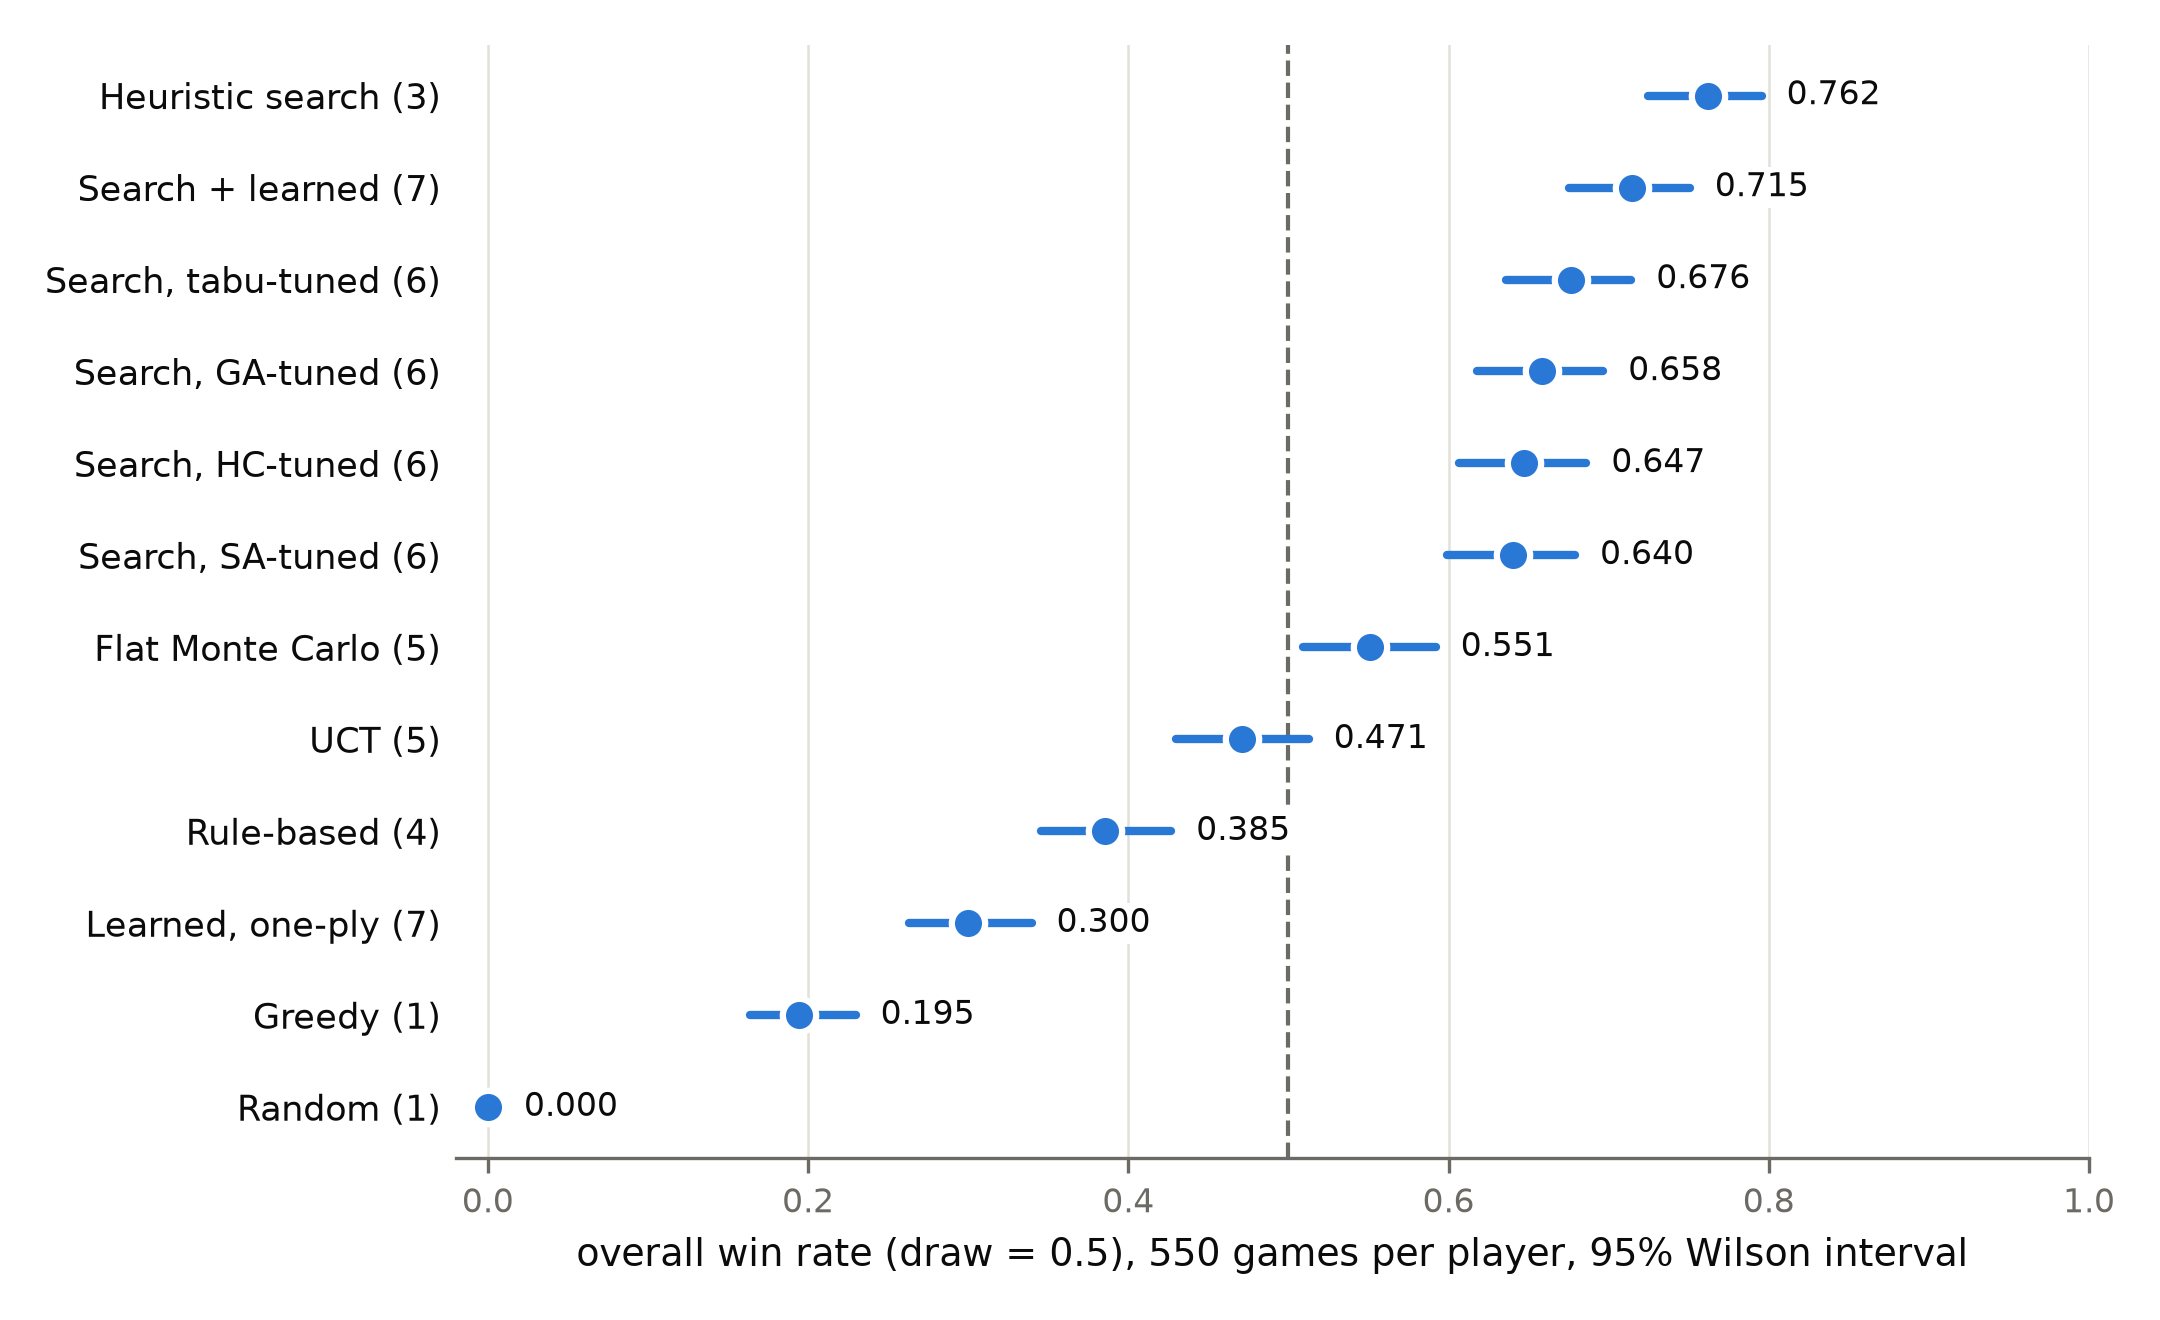
\includegraphics[width=0.88\linewidth]{e1_strength.png}
\caption{E1: overall win rate of each player in the \bd{3}{3} round robin with its 95\% Wilson
interval (550 games per player); the solver number is in brackets. The dashed line marks 0.5.}
\label{fig:e1}
\end{figure}

The search-based players form the top tier (Figure~\ref{fig:e1}). Untuned search reached a
mean depth of 8.2 plies with about 26{,}000 nodes per move and $b^*=2.56$. No game was drawn:
nine boxes cannot be split evenly. At 50 games per pair, untuned search,
search with the learned evaluation and the tabu-tuned player cannot be separated
head-to-head (search scores 0.50 [0.37, 0.63] against search-learned and 0.54 [0.40,
0.67] against tabu). Search scores at least 0.80 against every non-search player. The result
set contains a non-transitive cycle: flat Monte Carlo beats UCT (0.64), UCT beats the rule
player (0.64), and flat Monte Carlo only ties the rule player (0.50). The rule player
beats Greedy 0.86 and the one-ply learned player 1.00, but loses to every search player.

Table~\ref{tab:optimal} complements E1 with the share of optimal moves, judged by the exact
solver, on 60 positions per board from seeded self-play (on \bd{3}{3} restricted to
positions with at most 18 undrawn edges). Search remains near-perfect on all three
boards, while the rule player and Greedy fall to about two-thirds on late \bd{3}{3}
positions.

\begin{table}[htbp]
\centering
\caption{Share of optimal moves against the exact solver (60 positions per board, seed 7,
1\,s per move).}
\label{tab:optimal}
\begin{tabular}{lccc}
\toprule
Player & \bd{2}{2} & \bd{2}{3} & \bd{3}{3} (late game) \\
\midrule
Heuristic search & 100\% & 100\% & 96.7\% \\
Search + learned & -- & 96.7\% & 95.0\% \\
Search, GA-tuned & -- & -- & 96.7\% \\
Search, tabu / SA / HC-tuned & -- & -- & 93.3\% \\
Flat Monte Carlo & 93.3\% & 90.0\% & 86.7\% \\
UCT & 100\% & 83.3\% & 81.7\% \\
Rule-based & 85.0\% & 81.7\% & 68.3\% \\
Greedy & 85.0\% & 81.7\% & 65.0\% \\
Learned, one-ply & -- & 81.7\% & 65.0\% \\
Random & 53.3\% & 65.0\% & 28.3\% \\
\bottomrule
\end{tabular}
\end{table}

\FloatBarrier
\subsection{E2: Search efficiency}

Table~\ref{tab:e2exact} gives the nodes the exact solver expands to solve the empty board.
Memoisation is the decisive step: on \bd{1}{3} it cuts the nodes of plain negamax by a
factor of 1{,}926. Plain memoisation visits exactly $E\cdot 2^{E-1}+1$ nodes (on \bd{2}{3},
$17\cdot 2^{16}+1 = 1{,}114{,}113$): one root call plus one call for every pair of a position
and one of its undrawn edges, as the bound of Section~\ref{sec:method} predicts. Symmetry
reduction saves $7.2\times$ on the square \bd{2}{2} board and $3.9\times$ on \bd{2}{3}, close
to their 8 and 4 symmetries. On \bd{2}{3}, alpha-beta saves $4.8\times$ and both refinements
together $8.8\times$. Nodes and time disagree for symmetry: on \bd{2}{3}
alpha-beta takes 0.078\,s and alpha-beta with symmetry 0.114\,s, because computing the
canonical form costs more than the nodes it saves at this size. With alpha-beta and
symmetry the solver also solves \bd{3}{3} (13.7 million nodes, 42\,s): the first player
loses by three boxes under perfect play, $V=-3$.

\begin{table}[htbp]
\centering
\caption{E2, solver 2: nodes expanded to solve the empty board; every method returns the
same value. Brute force (no memo) is run only up to 10 edges.}
\label{tab:e2exact}
\begin{tabular}{lrrrrrr}
\toprule
Board & Brute force & Memo & Memo+sym & Alpha-beta & Alpha-beta+sym & $V(\text{empty})$ \\
\midrule
\bd{1}{2} & 13{,}700 & 449 & 169 & 305 & 141 & 0 \\
\bd{1}{3} & 9{,}864{,}101 & 5{,}121 & 1{,}561 & 2{,}021 & 1{,}160 & $-1$ \\
\bd{2}{2} & -- & 24{,}577 & 3{,}421 & 8{,}363 & 2{,}522 & $+2$ \\
\bd{2}{3} & -- & 1{,}114{,}113 & 283{,}969 & 232{,}394 & 127{,}159 & $-2$ \\
\bottomrule
\end{tabular}
\end{table}

Table~\ref{tab:e2search} ablates solver 3 on 40 \bd{3}{3} positions from seeded Greedy
self-play. Move ordering is the largest single saving ($6.6\times$ fewer nodes at depth
6), followed by the transposition table ($2.8\times$); with all enhancements off the
search needs $14.9\times$ the nodes. The savings grow with depth: at depth 2 the table makes
no difference. Under a 1\,s limit the full player searches about four
plies deeper than the stripped one (10.3 against 6.0). Turning quiescence \emph{off}
reduces the nodes ($0.76\times$): quiescence extends capture sequences at the leaves, so it
costs nodes and buys evaluation accuracy rather than speed.

\begin{table}[htbp]
\centering
\caption{E2, solver 3: mean nodes per position at fixed depth (ratio to the full player
in brackets), $b^*$ at depth 6, and mean depth reached in 1\,s; 40 \bd{3}{3} positions,
seed 0.}
\label{tab:e2search}
\small
\begin{tabular}{lrrrrr}
\toprule
Configuration & Depth 2 & Depth 4 & Depth 6 & $b^*$ at depth 6 & Depth in 1\,s \\
\midrule
Full & 119 & 1{,}397 & 11{,}203 & 4.10 & 10.32 \\
No transposition table & 119 (1.00) & 1{,}681 (1.20) & 31{,}364 (2.80) & 4.80 & 8.68 \\
No move ordering & 243 (2.05) & 6{,}508 (4.66) & 73{,}970 (6.60) & 5.92 & 8.38 \\
No quiescence & 64 (0.54) & 1{,}013 (0.73) & 8{,}461 (0.76) & 3.76 & 10.20 \\
None of the three & 93 (0.78) & 3{,}832 (2.74) & 166{,}758 (14.88) & 6.47 & 5.97 \\
\bottomrule
\end{tabular}
\end{table}

\FloatBarrier
\subsection{E3: Optimiser comparison}

Figure~\ref{fig:e3} shows the best fitness found against the number of fitness evaluations
on \bd{3}{3}, averaged over three seeds. Tabu search and the GA climb fastest and end
highest; hill climbing and simulated annealing improve more slowly.
Table~\ref{tab:e3} lists the final fitness per seed and the re-evaluation of each
optimiser's best weights against untuned search on 400 fresh games at the tuning depth.
All four tuned players beat untuned search with the confidence interval above 0.5. Tabu,
the GA and simulated annealing cannot be separated; hill climbing's interval lies entirely
below the other three, so it is significantly weaker. Tabu's $\pm0.5$ steps often revisit weight vectors, which
the fitness cache answers instantly, so its runs took about 4.5 minutes against about
13 for the GA and hill climbing, at the same budget of evaluations.

\begin{figure}[htbp]
\centering
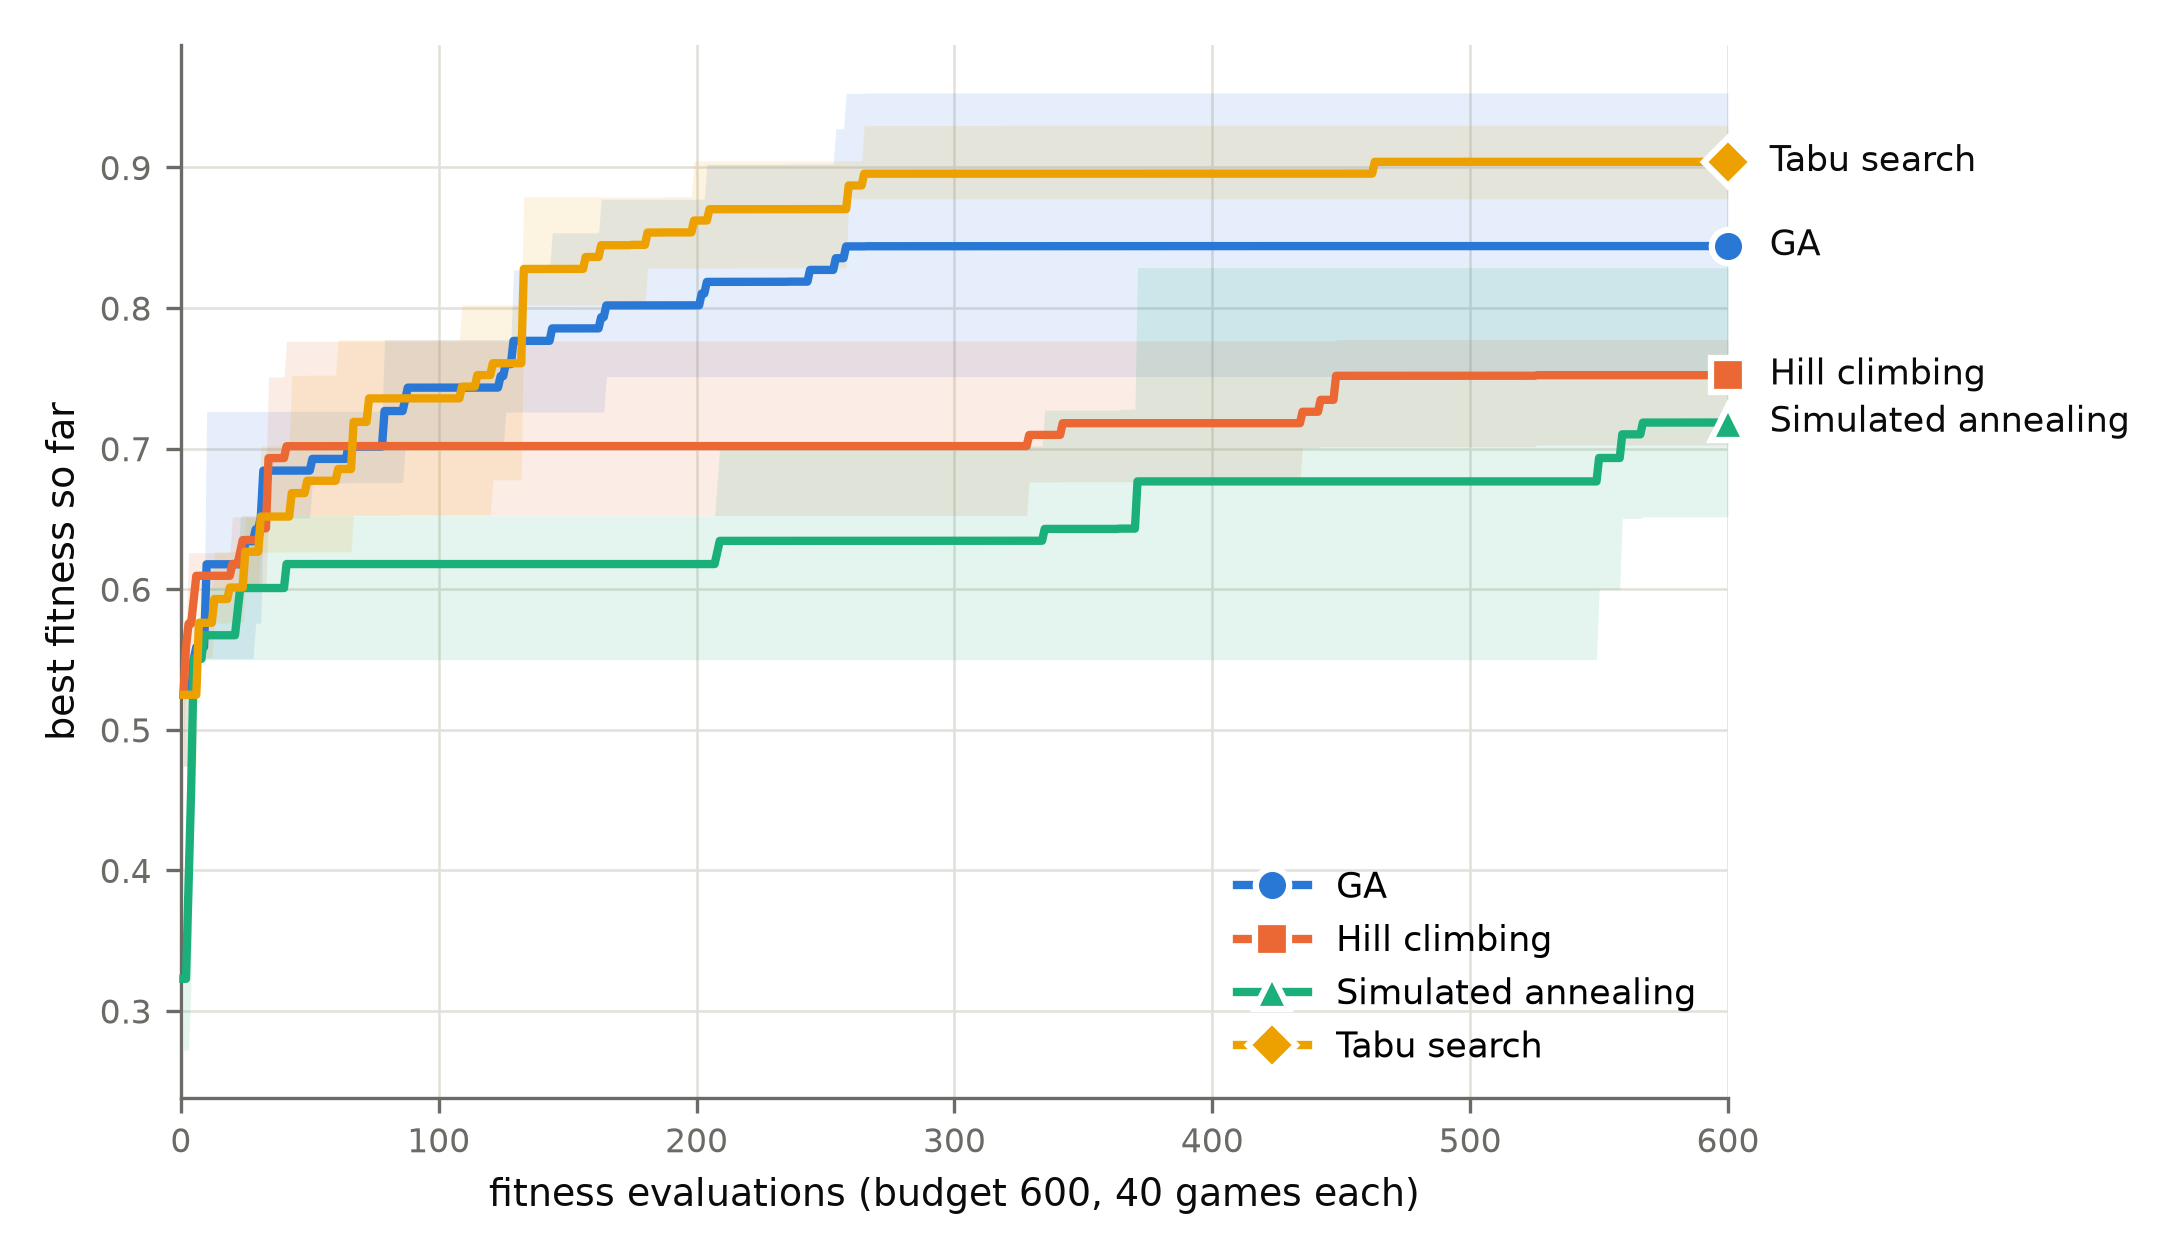
\includegraphics[width=0.92\linewidth]{e3_traces.png}
\caption{E3: best fitness so far against fitness evaluations on \bd{3}{3} (600-evaluation
budget, 40 games per evaluation). Lines are the mean over seeds 0--2; shaded bands span
the three seeds.}
\label{fig:e3}
\end{figure}

\begin{table}[htbp]
\centering
\caption{E3 on \bd{3}{3}: best fitness per seed after 600 evaluations, and the best
weights re-evaluated on 400 fresh games against untuned search, both at depth 2.}
\label{tab:e3}
\begin{tabular}{lccccc}
\toprule
 & \multicolumn{4}{c}{Best fitness} & Re-evaluation \\
\cmidrule(lr){2-5}
Optimiser & Seed 0 & Seed 1 & Seed 2 & Mean & win rate [95\% CI], margin \\
\midrule
Tabu search & 0.930 & 0.878 & 0.904 & 0.904 & 0.760 [0.716, 0.799], $+2.56$ \\
Genetic algorithm & 0.828 & 0.751 & 0.953 & 0.844 & 0.750 [0.705, 0.790], $+1.59$ \\
Hill climbing & 0.703 & 0.777 & 0.778 & 0.752 & 0.633 [0.584, 0.678], $+0.91$ \\
Simulated annealing & 0.676 & 0.829 & 0.651 & 0.719 & 0.733 [0.687, 0.774], $+2.48$ \\
\bottomrule
\end{tabular}
\end{table}

\paragraph{The gain does not survive deeper search.} In E1, played at 1\,s per move with
iterative deepening, every tuned player ranks \emph{below} untuned search (0.64--0.68
against 0.76), and untuned search beats them head-to-head (0.54 against tabu up to 0.68
against hill climbing). The tuned players also stop searching earlier (98--121\,ms per
move against 186\,ms) and search about one ply less deep (7.0--7.2 plies against 8.2) with a
higher effective branching factor ($b^*$ 3.6--4.0 against 2.6): weights optimised only for
depth-2 play are a concrete case of overfitting an evaluation function to the conditions
of its fitness function.

\paragraph{Why tuned weights break on larger boards.} When the same tuning is run
separately on \bd{3}{4}, \bd{4}{4} and \bd{5}{5} (Section~\ref{sec:boards}), the tuned
players reach best fitness of 0.79--0.98 at depth 2 but collapse at 1\,s per move: on \bd{5}{5}
they beat Greedy in only 3--48\% of games, while untuned search wins 88\%. With the
\bd{5}{5} tabu weights, the player wins 6 of 8 games against Greedy at depth 2, but only 2
of 8 at depth 4 or at 1\,s per move. The cause is the value convention combined with
raw-count features. The tuned weights give real weight to counts that are large and the
same for both players: the \bd{5}{5} tabu weights put $1.0$ on the number of safe moves (60
at the start) and $0.5$ on untouched boxes (25), so $h(s)$ is about $\pm70$ boxes, against
about $\pm2.5$ for the hand-set weights. At depth 2 the leaves being compared usually have
the same player to move, so this common term cancels. In deeper search, captures give
extra turns, so the compared leaves differ in who is to move, and the search chooses
lines by the $\pm70$ sign flip instead of by real boxes worth one each: it gives boxes
away. Larger boards have larger counts, so the effect grows with board size. Two checks
confirm the mechanism: keeping only the parity and capturable-box weights restores the
\bd{5}{5} players at 1\,s per move (tabu 0.025 $\rightarrow$ 0.700, GA 0.225 $\rightarrow$
0.800 against Greedy over 20 games), and so does playing them at their tuning depth of 2
(0.83--0.95 over 40 games). For the same
reason, weights tuned on \bd{3}{3} do not transfer: on 25 \bd{5}{5} positions the
tabu-tuned \bd{3}{3} weights gave a box away in 19 and the GA weights in 16, against none
for untuned search. Fitness should therefore be measured at the depth used in play, and
count features should be normalised by board size.

\FloatBarrier
\subsection{E4: Learned evaluators}

The \bd{2}{3} dataset holds 32{,}622 positions from 15{,}764 games with exact labels
(22{,}756 / 4{,}920 / 4{,}946 for training, validation and test); the \bd{3}{3} dataset holds
50{,}000 positions from 4{,}344 games with Monte Carlo labels (7{,}559 for test).
Table~\ref{tab:e4opt} gives the share of optimal one-ply moves on the \bd{2}{3} test set,
whose positions come from games never seen in training, and Table~\ref{tab:e4err} the
test error on both boards. The two-hidden-layer MLP on both inputs is best everywhere: 97.2\% optimal
moves on \bd{2}{3} (test MSE 0.024) and test MSE 0.041 on \bd{3}{3}. With their best input,
kNN with $k=15$, both MLPs, the SVM and the tree beat Greedy's 89.4\% on \bd{2}{3}; the
perceptron, the sigmoid unit, kNN with $k=1$ and naive Bayes do not. The
hand-made features $\phi$ help the simple learners most (kNN, tree, sigmoid unit), while
only the MLP makes good use of the raw edge bits: on raw input alone it reaches 95.0\%, a
sign that it learns structure the 12 features do not capture. Regression transfers better
to move choice than classification: the same $64{\times}64$ network trained as a classifier
picks an optimal move in only 80.4\% of positions, because a win/loss label does not rank
one winning move above another. The linear models cannot
represent the game well: the perceptron misclassifies 15.1\% of \bd{2}{3} test positions
($\phi$) and 24.4\% on \bd{3}{3}, against 8.7\% and 8.5\% sign errors for the MLP.

\begin{table}[htbp]
\centering
\caption{E4: optimal one-ply moves on the \bd{2}{3} test set, by model and input
(regression models, except the perceptron and naive Bayes, which are classifiers).
Greedy reaches 89.4\%, Random 29.9\%.}
\label{tab:e4opt}
\begin{tabular}{lccc}
\toprule
Model & $\phi$ & Raw edges & Both \\
\midrule
kNN, $k=1$ & 86.9\% & 83.0\% & 87.6\% \\
kNN, $k=15$ & 93.7\% & 88.8\% & 91.1\% \\
Perceptron (from scratch) & 84.5\% & 83.8\% & 83.8\% \\
Sigmoid unit (from scratch) & 88.5\% & 83.5\% & 87.8\% \\
MLP, 64 & 93.3\% & 92.9\% & 94.0\% \\
MLP, $64{\times}64$ & 93.8\% & 95.0\% & \textbf{97.2\%} \\
SVM & 92.9\% & 88.9\% & 92.1\% \\
Naive Bayes & 79.7\% & 83.6\% & 79.7\% \\
Decision tree & 94.1\% & 84.0\% & 93.9\% \\
\bottomrule
\end{tabular}
\end{table}

\begin{table}[htbp]
\centering
\caption{E4: test mean squared error of the regression models.}
\label{tab:e4err}
\begin{tabular}{lcccccc}
\toprule
 & \multicolumn{3}{c}{\bd{2}{3} (exact labels)} & \multicolumn{3}{c}{\bd{3}{3} (Monte Carlo labels)} \\
\cmidrule(lr){2-4}\cmidrule(lr){5-7}
Model & $\phi$ & Raw & Both & $\phi$ & Raw & Both \\
\midrule
kNN, $k=1$ & 0.098 & 0.149 & 0.090 & 0.144 & 0.317 & 0.161 \\
kNN, $k=15$ & 0.063 & 0.093 & 0.068 & 0.081 & 0.165 & 0.094 \\
Sigmoid unit & 0.108 & 0.190 & 0.109 & 0.165 & 0.203 & 0.166 \\
MLP, 64 & 0.060 & 0.057 & 0.045 & 0.079 & 0.074 & 0.056 \\
MLP, $64{\times}64$ & 0.057 & 0.036 & \textbf{0.024} & 0.074 & 0.060 & \textbf{0.041} \\
SVM & 0.065 & 0.086 & 0.056 & 0.089 & 0.119 & 0.092 \\
Decision tree & 0.058 & 0.174 & 0.058 & 0.076 & 0.153 & 0.087 \\
\bottomrule
\end{tabular}
\end{table}

\paragraph{Bias and variance.} Figure~\ref{fig:bv} varies the hidden layer of a one-layer
MLP on \bd{2}{3} (raw input, 10\% of the training games, three seeds). Without
regularisation, the test MSE rises from 0.104 at 2 units to 0.133 at 256 units while the
training MSE falls to 0.002: high variance (overfitting). With L2 and early stopping, the
test MSE stays at 0.104--0.109 for every size. A single unit underfits in both regimes
(training 0.171, test 0.174): high bias. The spread across seeds is at most 0.0034.

\begin{figure}[htbp]
\centering
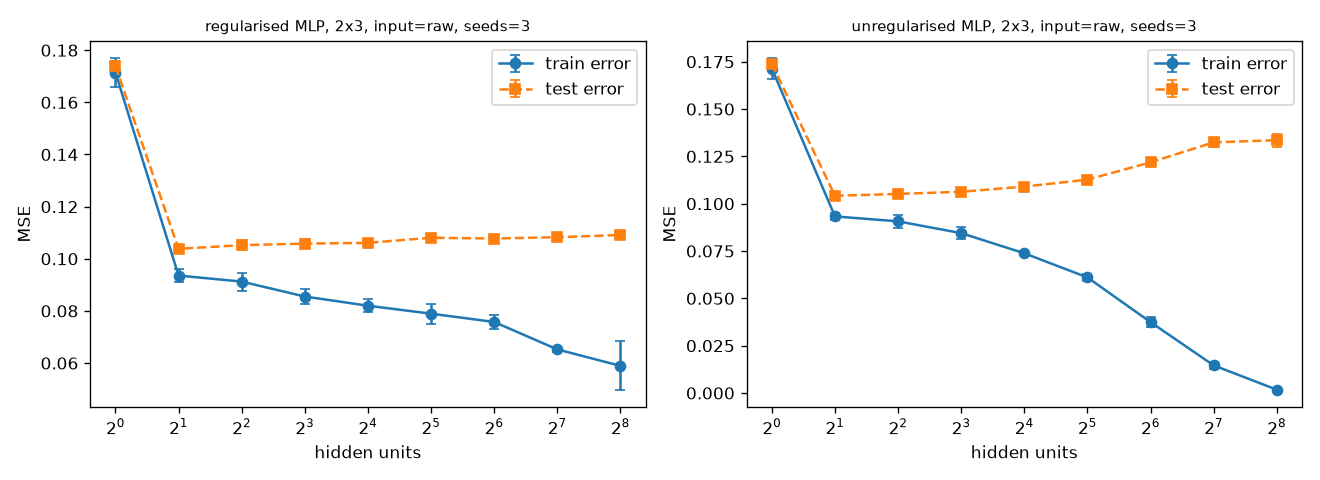
\includegraphics[width=0.9\linewidth]{e4_bias_variance.png}
\caption{E4 bias--variance: train and test MSE against hidden-layer size on \bd{2}{3}, without
(left) and with (right) L2 and early stopping; mean and standard deviation over three
seeds.}
\label{fig:bv}
\end{figure}

\FloatBarrier
\subsection{E5: Deductive against inductive play}

E5 pits the rule player against the learned players and Greedy in round robins of 200
games per pair (Table~\ref{tab:e5}). On \bd{2}{3}, where the model was trained on exact
values, the one-ply learned player and the rule player tie (0.500); both beat Greedy (0.685
and 0.665), and against the perfect exact player the learned player holds up better (0.488
against 0.325). On \bd{3}{3}, the one-ply
learned player still beats Greedy (0.605 [0.536, 0.670]) but never beats the rule player
(0.000): one move of lookahead cannot see the chain endgame that the rules encode.
Inside search, however, the learned evaluation beats the rules 0.990 and Greedy 0.970.
Deduction encodes the endgame exactly but has no lookahead; induction provides a good
static estimate, and search turns it into strong play.

\begin{table}[htbp]
\centering
\caption{E5: head-to-head win rate of the row player (200 games per pair, 1.0\,s per move,
seed 0). Models: MLP $64{\times}64$, both inputs, regression, trained on the same board.}
\label{tab:e5}
\begin{tabular}{llc}
\toprule
Board & Match & Win rate [95\% CI] \\
\midrule
\multirow{5}{*}{\bd{2}{3}} & Learned (one-ply) vs rule-based & 0.500 \\
 & Learned (one-ply) vs Greedy & 0.685 \\
 & Rule-based vs Greedy & 0.665 \\
 & Learned (one-ply) vs exact & 0.488 \\
 & Rule-based vs exact & 0.325 \\
\midrule
\multirow{5}{*}{\bd{3}{3}} & Learned (one-ply) vs Greedy & 0.605 [0.536, 0.670] \\
 & Learned (one-ply) vs rule-based & 0.000 \\
 & Search + learned vs rule-based & 0.990 [0.964, 0.997] \\
 & Search + learned vs Greedy & 0.970 [0.936, 0.986] \\
 & Rule-based vs Greedy & 0.845 \\
\bottomrule
\end{tabular}
\end{table}

\FloatBarrier
\subsection{E6: Monte Carlo scaling}

Figure~\ref{fig:e6} and Table~\ref{tab:e6} show the win rate against Greedy on \bd{3}{3} as the
number of iterations per move grows (100 games per point, the same game seeds at every
point). UCT improves with budget (0.21 $\rightarrow$ 0.67) but passes 0.5 only from 3{,}000
iterations, whereas flat Monte Carlo is at 0.74 from 100 iterations and saturates at 0.99.
Greedy rollouts beat random rollouts at every budget, and the conclusions also hold at
equal time per move: UCT with random rollouts at 10{,}000 iterations (311\,ms) scores 0.37
against 0.54 for Greedy rollouts at 3{,}000 (193\,ms), and flat Monte Carlo at 1{,}000
iterations (58\,ms) scores 0.94 against 0.24 for UCT at the same budget (53\,ms).

\begin{figure}[htbp]
\centering
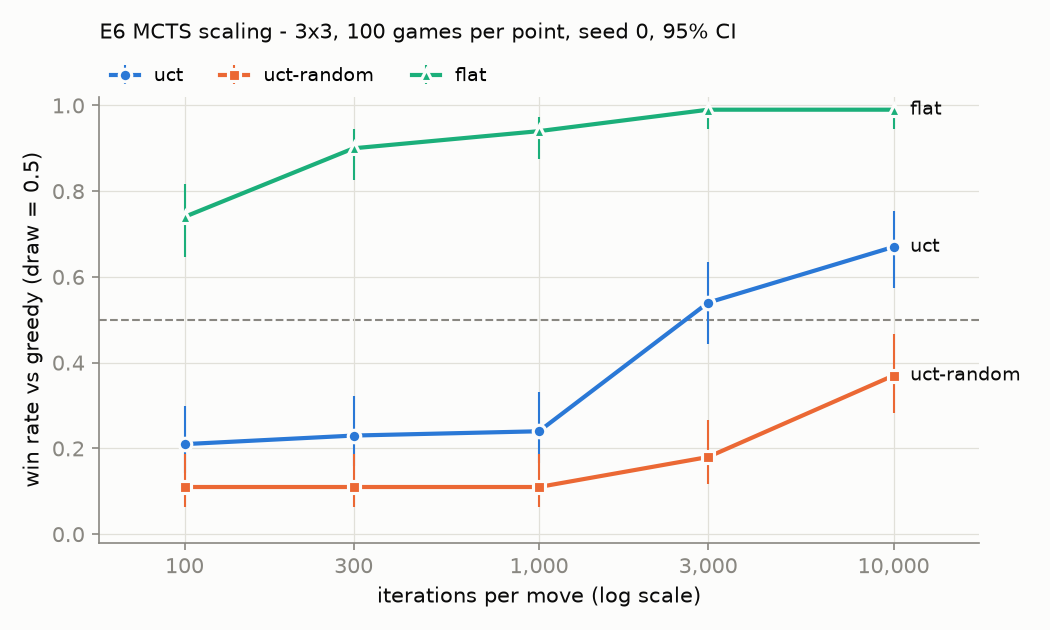
\includegraphics[width=0.85\linewidth]{e6_mcts_scaling.png}
\caption{E6: win rate against Greedy on \bd{3}{3} against iterations per move (log scale), 100
games per point, 95\% Wilson intervals.}
\label{fig:e6}
\end{figure}

\begin{table}[htbp]
\centering
\caption{E6: win rate against Greedy and mean time per move on \bd{3}{3} (100 games per
point, seed 0).}
\label{tab:e6}
\begin{tabular}{rccc}
\toprule
Iterations & UCT, Greedy rollouts & UCT, random rollouts & Flat, Greedy rollouts \\
\midrule
100 & 0.21 (4\,ms) & 0.11 (3\,ms) & 0.74 (6\,ms) \\
300 & 0.23 (12\,ms) & 0.11 (10\,ms) & 0.90 (17\,ms) \\
1{,}000 & 0.24 (53\,ms) & 0.11 (32\,ms) & 0.94 (58\,ms) \\
3{,}000 & 0.54 (193\,ms) & 0.18 (96\,ms) & 0.99 (173\,ms) \\
10{,}000 & 0.67 (590\,ms) & 0.37 (311\,ms) & 0.99 (568\,ms) \\
\bottomrule
\end{tabular}
\end{table}

We traced UCT's weakness to the rollout policy. Greedy rollouts never double-deal: the
player in control takes every box and must then hand boxes back, so averaged backups
through long capture sequences learn the double-deal only slowly. On 60 \bd{3}{3}
endgame positions scored by the exact solver, at 2{,}000 iterations flat Monte Carlo chose an
optimal move in 78\% of positions and UCT in only 55\%; UCT needed 20{,}000 iterations to
reach 77\%. Flat Monte Carlo makes the
same rollout error for every root move, so its ranking of moves stays correct, while the
tree compounds the error. A double-dealing rollout policy, exact endgame solving or
solver-style backups are natural fixes \cite{browne2012survey,zhuang2015dotsboxes}.

\FloatBarrier
\subsection{Larger boards}
\label{sec:boards}

To offer every player on \bd{3}{4}, \bd{4}{4} and \bd{5}{5} in an interactive application,
each one was optimised per board (tuned weights, MCTS settings chosen from a small grid
on 30 games, and an MLP trained on 50{,}000 Monte Carlo-labelled positions per board) and
tested against Greedy (Table~\ref{tab:boards}). Flat Monte Carlo, untuned search,
search-learned and the rule player stay strong as the board grows; the rule player even
improves, most likely because larger boards have more and longer chains to control. UCT
collapses (0.075 on \bd{5}{5}): one second buys fewer iterations over a larger branching
factor, and the rollout error analysed in E6 compounds. The one-ply learned player falls
below Greedy beyond \bd{3}{3}, likely because its Monte Carlo labels become noisier and the
positions more varied. The tuned players collapse at 1\,s per move for the reason analysed in E3, and
recover when played at their tuning depth.

\begin{table}[htbp]
\centering
\caption{Win rate against Greedy on larger boards (40 games per entry, 1.0\,s per move,
seed 0). Tuned players are shown at 1\,s per move and at their tuning depth of 2.}
\label{tab:boards}
\small
\begin{tabular}{lccc}
\toprule
Player & \bd{3}{4} & \bd{4}{4} & \bd{5}{5} \\
\midrule
Flat Monte Carlo & 0.975 & 0.963 & 1.000 \\
Heuristic search & 0.913 & 0.913 & 0.875 \\
Search + learned & 0.875 & 0.863 & 0.725 \\
Rule-based & 0.738 & 0.900 & 0.950 \\
UCT & 0.763 & 0.525 & 0.075 \\
Learned, one-ply & 0.463 & 0.350 & 0.225 \\
\midrule
\multicolumn{4}{l}{\emph{Tuned players: at 1\,s per move / at depth 2}} \\
GA-tuned & 0.76 / 0.68 & 0.40 / 0.74 & 0.23 / 0.95 \\
Hill-climbing-tuned & 0.79 / 0.73 & 0.48 / 0.65 & 0.48 / 0.85 \\
SA-tuned & 0.76 / 0.86 & 0.46 / 0.71 & 0.08 / 0.83 \\
Tabu-tuned & 0.85 / 0.78 & 0.68 / 0.76 & 0.03 / 0.85 \\
\bottomrule
\end{tabular}
\end{table}

% ---------------------------------------------------------------- conclusion
\FloatBarrier
\section{Conclusion}

We implemented seven Dots and Boxes players covering exhaustive search, heuristic search,
knowledge representation, Monte Carlo methods, metaheuristic optimisation and supervised
learning, all on one engine with a value convention that handles the extra-turn rule.
The main findings are:
\begin{itemize}
\item \textbf{Search wins.} Iterative-deepening alpha-beta with a two-term hand-set
  evaluation is the strongest player on \bd{3}{3} and stays strong on every larger board
  we tested; move ordering and the
  transposition table let it search about four plies deeper per second. The first player
  loses \bd{3}{3} by three boxes under perfect play.
\item \textbf{Tuning must match its use.} Every metaheuristic improved the evaluation at
  the depth it was tuned at, with tabu search, the GA and simulated annealing
  indistinguishable and hill climbing weaker. The gain disappears in deeper search, and
  weights on raw counts break down on larger boards because a large term shared by both
  players flips sign with the player to move.
\item \textbf{Learning works, with lookahead.} A $64{\times}64$ MLP reaches 97.2\% optimal
  moves on \bd{2}{3} and learns from raw edges what the hand-made features miss, but a
  one-move learned player loses every game to the rule player on \bd{3}{3}; the same
  network inside search is the second-strongest player overall.
\item \textbf{Rollout policy matters more than the tree.} Flat Monte Carlo beats UCT at
  every budget on \bd{3}{3}, because Greedy rollouts never double-deal.
\end{itemize}

\paragraph{Limitations.}
\begin{itemize}
\item Everything is pure Python: the exact solver stops at \bd{3}{3}, so exact evaluation
  and exact labels exist only for small boards, and the Monte Carlo players get few
  iterations per second on large boards.
\item The search, rule and learned players compute long-chain parity assuming the player in
  seat 0 moved first. That holds in the harness and the application, but not for an
  arbitrary starting position.
\item Quiescence always captures, so search finds double-dealing only within its nominal
  depth, and the transposition table is cleared entirely when it fills up.
\item Tuned weights are specific to their tuning depth and board, and learned models to
  their training board; Monte Carlo labels estimate values under a Greedy rollout policy,
  not true game values.
\item Every experiment uses one seed setting and between 40 and 550 games per comparison, so
  close results (for example the top three players of E1) are not separable.
\end{itemize}

\paragraph{Future work.} Natural next steps are normalising the count features and measuring
fitness with time-limited games at the depth used in play; a double-dealing rollout policy,
exact endgame solving or guidance by the learned evaluator for MCTS; Nimstring values from
combinatorial game theory \cite{berlekamp2000dots} in place of the parity heuristic in
endgames; deeper or exact labels for the learned evaluators on larger boards; and
convolutional inputs, so that one model can serve several board sizes.

\paragraph{Reproducibility.} The code, every result file and the commands to regenerate
them are in the project repository. Every experiment is seeded, and each result row
records its seed, board and number of games.

% ---------------------------------------------------------------- references
\bibliographystyle{ieeetr}
\bibliography{references}

\end{document}
